\subsection{Bypass components in GBT data path}
As shown in \autoref{fig:gbt-data-path}, we can bypass components in GBT
input/output path.

\begin{figure}[ht]
    \centering
    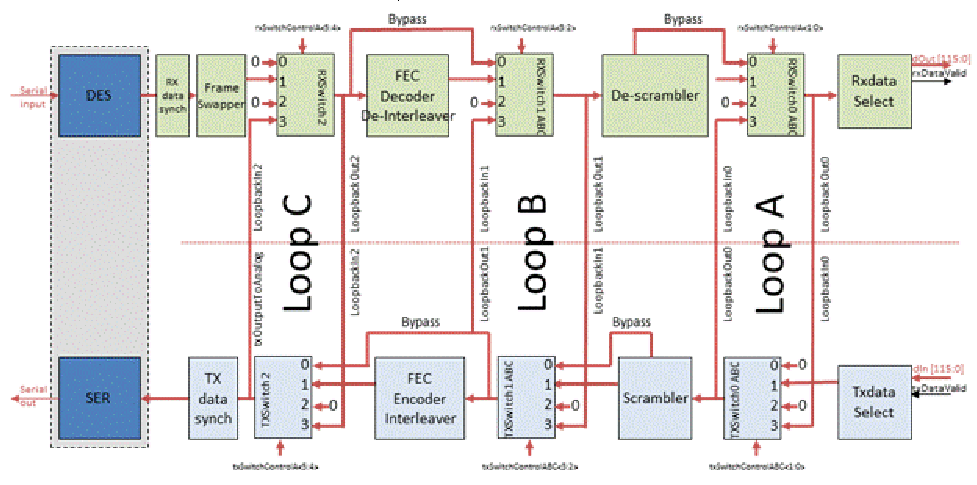
\includegraphics[width=\textwidth]{res/gbtx_data_path_block_diagram.pdf}
    \caption{GBT data path. Stolen from LHCb \emph{GBTX manual}.}
    \label{fig:gbt-data-path}
\end{figure}

The register \texttt{0x1c} and 3 subsequent registers control the output path;
\texttt{0x2d} controls the input path.
Each of the paths have 3 configurable selectors, each has 4 operations modes
($0_{10} - 3_{10}$\footnote{The subscript indicates the base.},
which translate to $0_2 - 11_2$). According to \autoref{fig:gbt-data-path}, the
control sequence should be given in:

\begin{lstlisting}
TXSwitch2 -> TXSwitch1 -> TXSwitch0
\end{lstlisting}

Here is an example.
Let us consider the Tx normal operating case (i.e.\ all 3 switches are
configured to 1). We have:
\begin{align*}
    \underbrace{1_{10}}_{\text{\tiny ~TXSwitch2~}}
    &\underbrace{1_{10}}_{\text{\tiny ~TXSwitch1~}}
    \underbrace{1_{10}}_{\text{\tiny ~TXSwitch0~}} \\
    &\symbolwithin{\Downarrow}{\text{\tiny ~TXSwitch0~}} \\
    \underbrace{01_{2}}_{\text{\tiny ~TXSwitch2~}}
    &\underbrace{01_{2}}_{\text{\tiny ~TXSwitch1~}}
    \underbrace{01_{2}}_{\text{\tiny ~TXSwitch0~}} \\
\end{align*}

To convert binary $010101_2$ to hexadecimal, we left pad the result with 2
additional 0's: $0001,0101_2$. The end result is $15_{16}$.

\begin{leftbar}
    $15_{16}$ is exactly the last 3 bytes in \textbf{Data out} field in
    \autoref{fig:gbt-i2c}.
    This is not a coincidence.
\end{leftbar}

\begin{leftbar}
    Recall that each 4 digits in binary exactly correspond to 1 digit in
    hexadecimal.
\end{leftbar}
